%!TEX root = ../dissertation.tex
\chapter{Gestione dei dati}


Prima di analizzare i dati è importante poter trovarli in modo efficiente ed efficace. Questo capitolo descrive i sistemi software implementati per la gestione dei dati, incluse operazioni come la ricerca rapida di specifici file raw in base a una o più condizioni, ma non affronta la lettura dei file stessi.

I file raw sono associati ai metadati disponibili nel foglio di calcolo di riferimento e nel file di configurazione del MPFM. Ogni file inoltre contiene nel nome la data in cui è stato creato nel formato \texttt{"YYYYmmdd hhmm"}

\section{Archiettura generale}
L'architettura del sistema di gestione dei dati può essere divisa in due parti principali. La prima parte si occupa di trovare e leggere i file di riferimento e configurazione per associare i metadati ai corretti file raw. La seconda parte si occupa di caricare tutte le informazioni raccolte in un database, per poter effettuare ricerche più complesse e veloci.
Navigare il sistema operativo esaustivamente per trovare tutti i file interessati è un'operazione temporalmente costosa, nell'ordine di una decina di minuti per le cartelle più grandi presenti nel server. Per migliorare il tempo di esecuzione vengono ricercati contemporaneamente tutti i tipi di file necessari, sia raw che di riferimento, invece di dover ripetere l'esplorazione più volte.
La ricerca deve essere sempre completa di tutte le sottocartelle in quanto i dati arrivano da molti laboratori diversi e la posizione dei file non rispetta uno standard uniforme.


\begin{figure}
	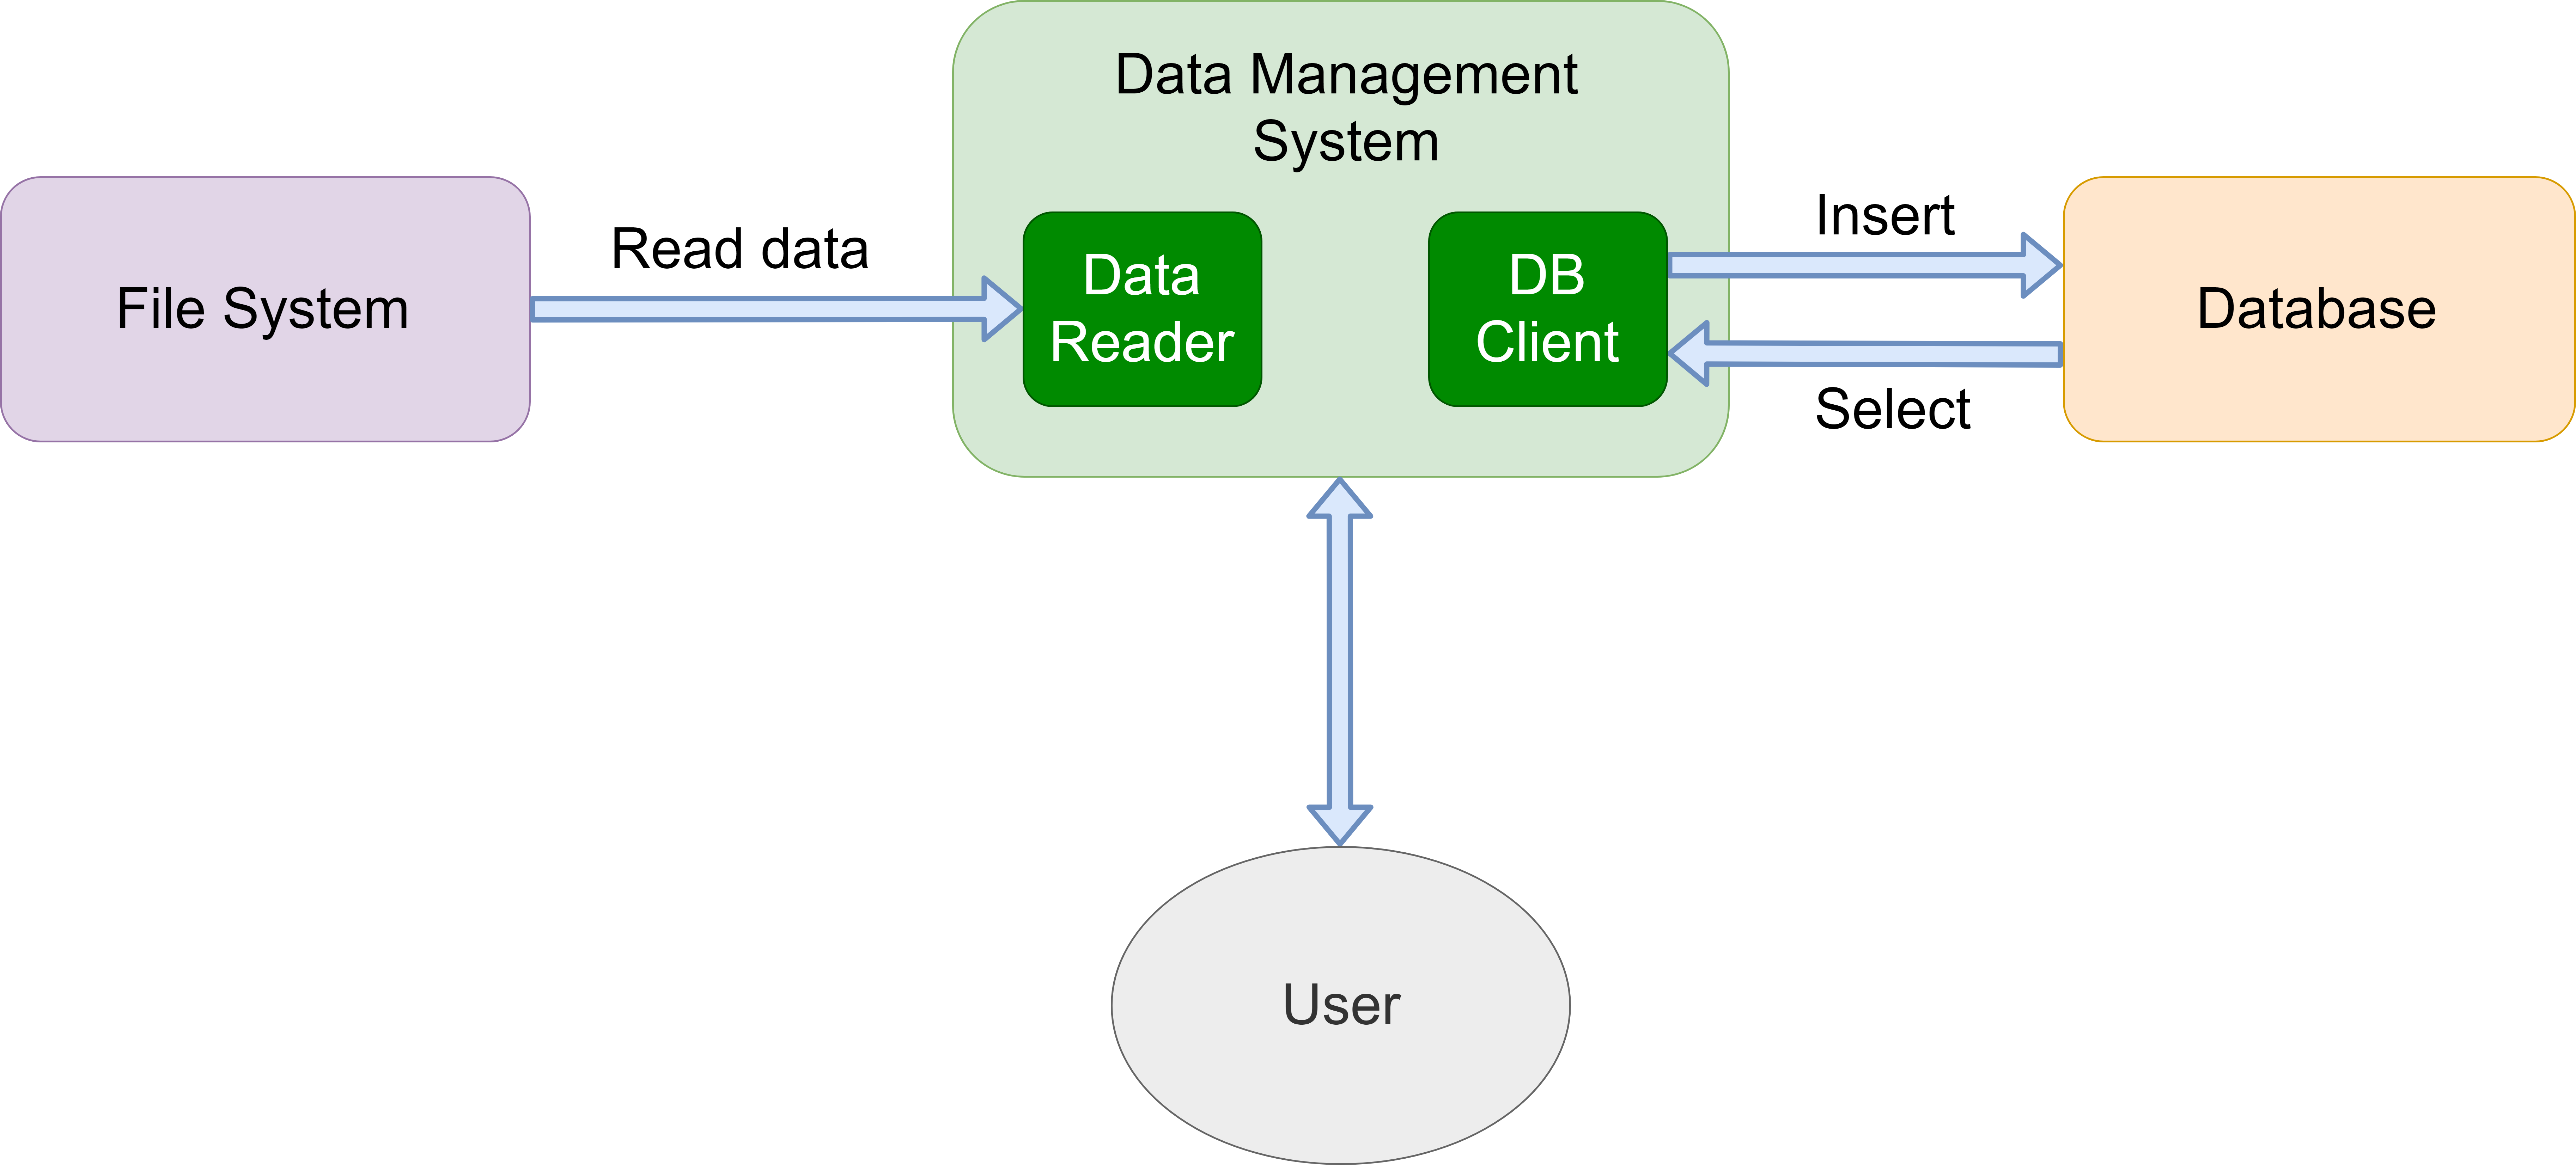
\includegraphics[width=\textwidth]{figures/ArchitetturaDMD}
	\caption[Architettura sistema di gestione dei dati]{Architettura generale del sistema di gestione dei dati e le interazioni verso le componenti esterne al sistema. 
		\label{fig:ArchietturaDMD}}
\end{figure}

\section{Diagramma delle classi} \label{DiagrammaDelleClassiDMD}

\begin{figure}
	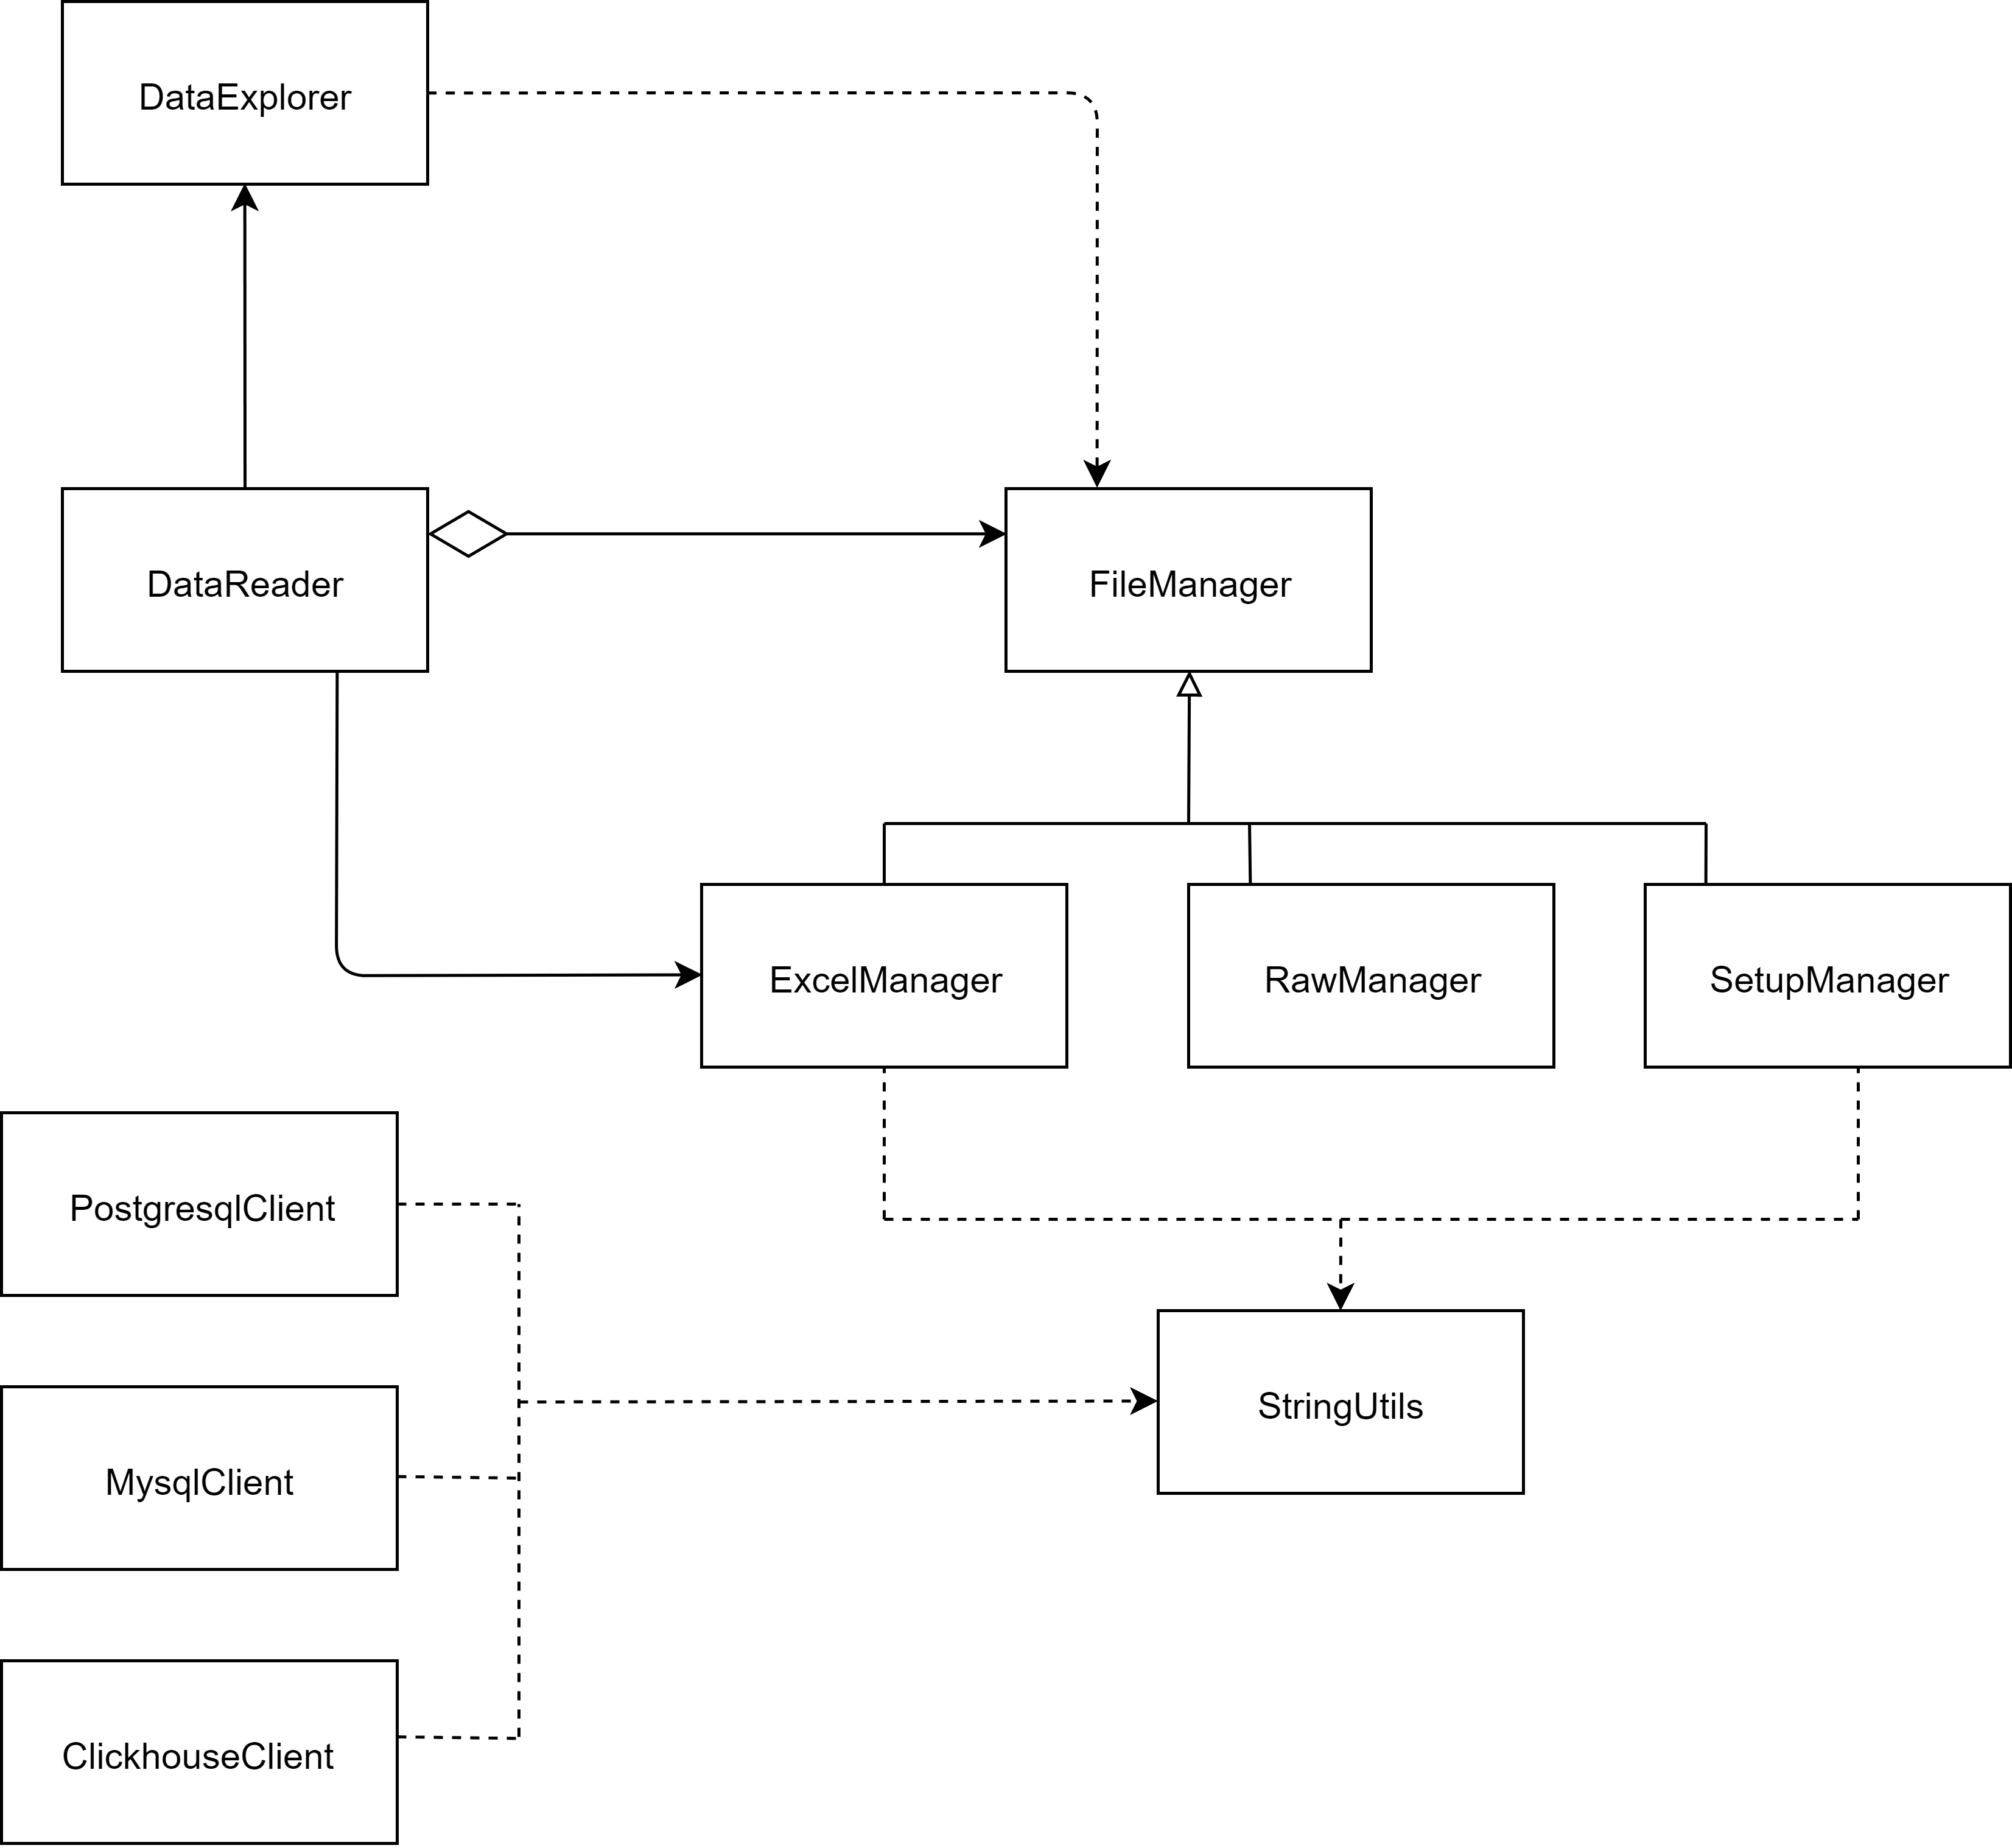
\includegraphics[width=\textwidth]{figures/DiagrammaDelleClassiDMD}
	\caption[Diagramma delle classi sistema di gestione dei dati]{Diagramma delle classi generale del sistema di gestione dei dati, rappresenta le dipendenze tra le classi senza entrare nei dettagli implementativi. 
		\label{fig:DiagrammaDelleClassiDMD}}
\end{figure}


DataReader è la classe principale del sistema di gestione dati e offre tutte le funzionalità necessarie per trovare i file e associarli con i relativi metadati.

ExcelManager, RawManager e SetupManager sono tre classi che gestiscono rispettivamente i file excel, i file raw, e file di testo di setup. Ognuno di questi Manager implementa due metodi fondamentali:

\begin{itemize}
	\item il metodo \texttt{match()} che dato il percorso e il nome di un file è in grado di riconoscere se è un file di interesse per quel manager, ad esempio ExcelManager ritornerà \texttt{True} solo se il file dato è l'excel di riferimento corretto.
	
	\item il metodo \texttt{get\_data()} che data la lista di file riconosciuti in precedenza per ognuno estrae le informazioni rilevanti, ad esempio SetupManager ricaverà i moduli installati in base al contenuto del file di testo. RawManager invece si occupa solo di estrarre la data e l'ora dal nome del file e non di leggere il contenuto del raw.
\end{itemize}

La sezione \ref{"StrutturaDeiDati"} affronta in più dettaglio la struttura dei file e il loro contenuto.

FileManager è una classe astratta che impone l'implementazione di questi due metodi a tutti i Manager che ereditano da essa e permette a DataReader di usarle polimorficamente senza sapere quali e quanti Manager sono presenti. Questa scelta implementativa è stata fatta per rendere facilmente estendibile il sistema, in particolare nell'aggiunta di nuovi Manager per altri tipi di file che si potrebbero voler analizzare in futuro.

DataExplorer è la classe usata per navigare il file system e sfrutta il metodo \texttt{match()} dei FileManager per costruire una lista di percorsi dei file rilevanti.

StringUtils è una semplice classe di utilità che contiene delle funzionalità comuni per manipolare ed elaborare stringhe.

PostgresqlClient, MysqlClient e ClickhouseClient sono delle classi per la comunicazione con il database. Mysql è il database scelto dall'azienda quindi per ora MysqlClient è l'unico utilizzato, le altre due classi hanno la stessa interfaccia e possono essere intercambiate liberamente se si volesse utilizzare un database diverso.
Tutti e tre i client offrono la possibilità di eseguire query SQL oppure creare tabelle e popolarle automaticamente attraverso il risultato ritornato da DataReader.


